\documentclass[10pt]{article}

\usepackage[skip=7pt plus1pt, indent=0pt]{parskip}
\usepackage{hyperref}
\usepackage[margin=0.7in]{geometry}
\usepackage{cite}
\usepackage{graphicx}
\usepackage{caption}
\usepackage{subcaption}
\usepackage{float}
\thispagestyle{empty}

\AtBeginDocument{%
  \providecommand\BibTeX{{%
    Bib\TeX}}}

\newcommand{\tall}{\phantom{\large PQq}}
\thispagestyle{empty}

\begin{document}
\thispagestyle{empty}

\vspace{-2em}
\title{\textsc{CMPE-258} Executive Summary: Hand-drawn Flowchart Recognition}
\date{}

\vspace{-2em}
\author{}
% \author{Mu Chen, Roger Kuo, Hardy Leung, Jasmine Wang}

\maketitle

\vspace{-5em}

\begin{figure}[h]
\centering
\begin{subfigure}{0.28\columnwidth}
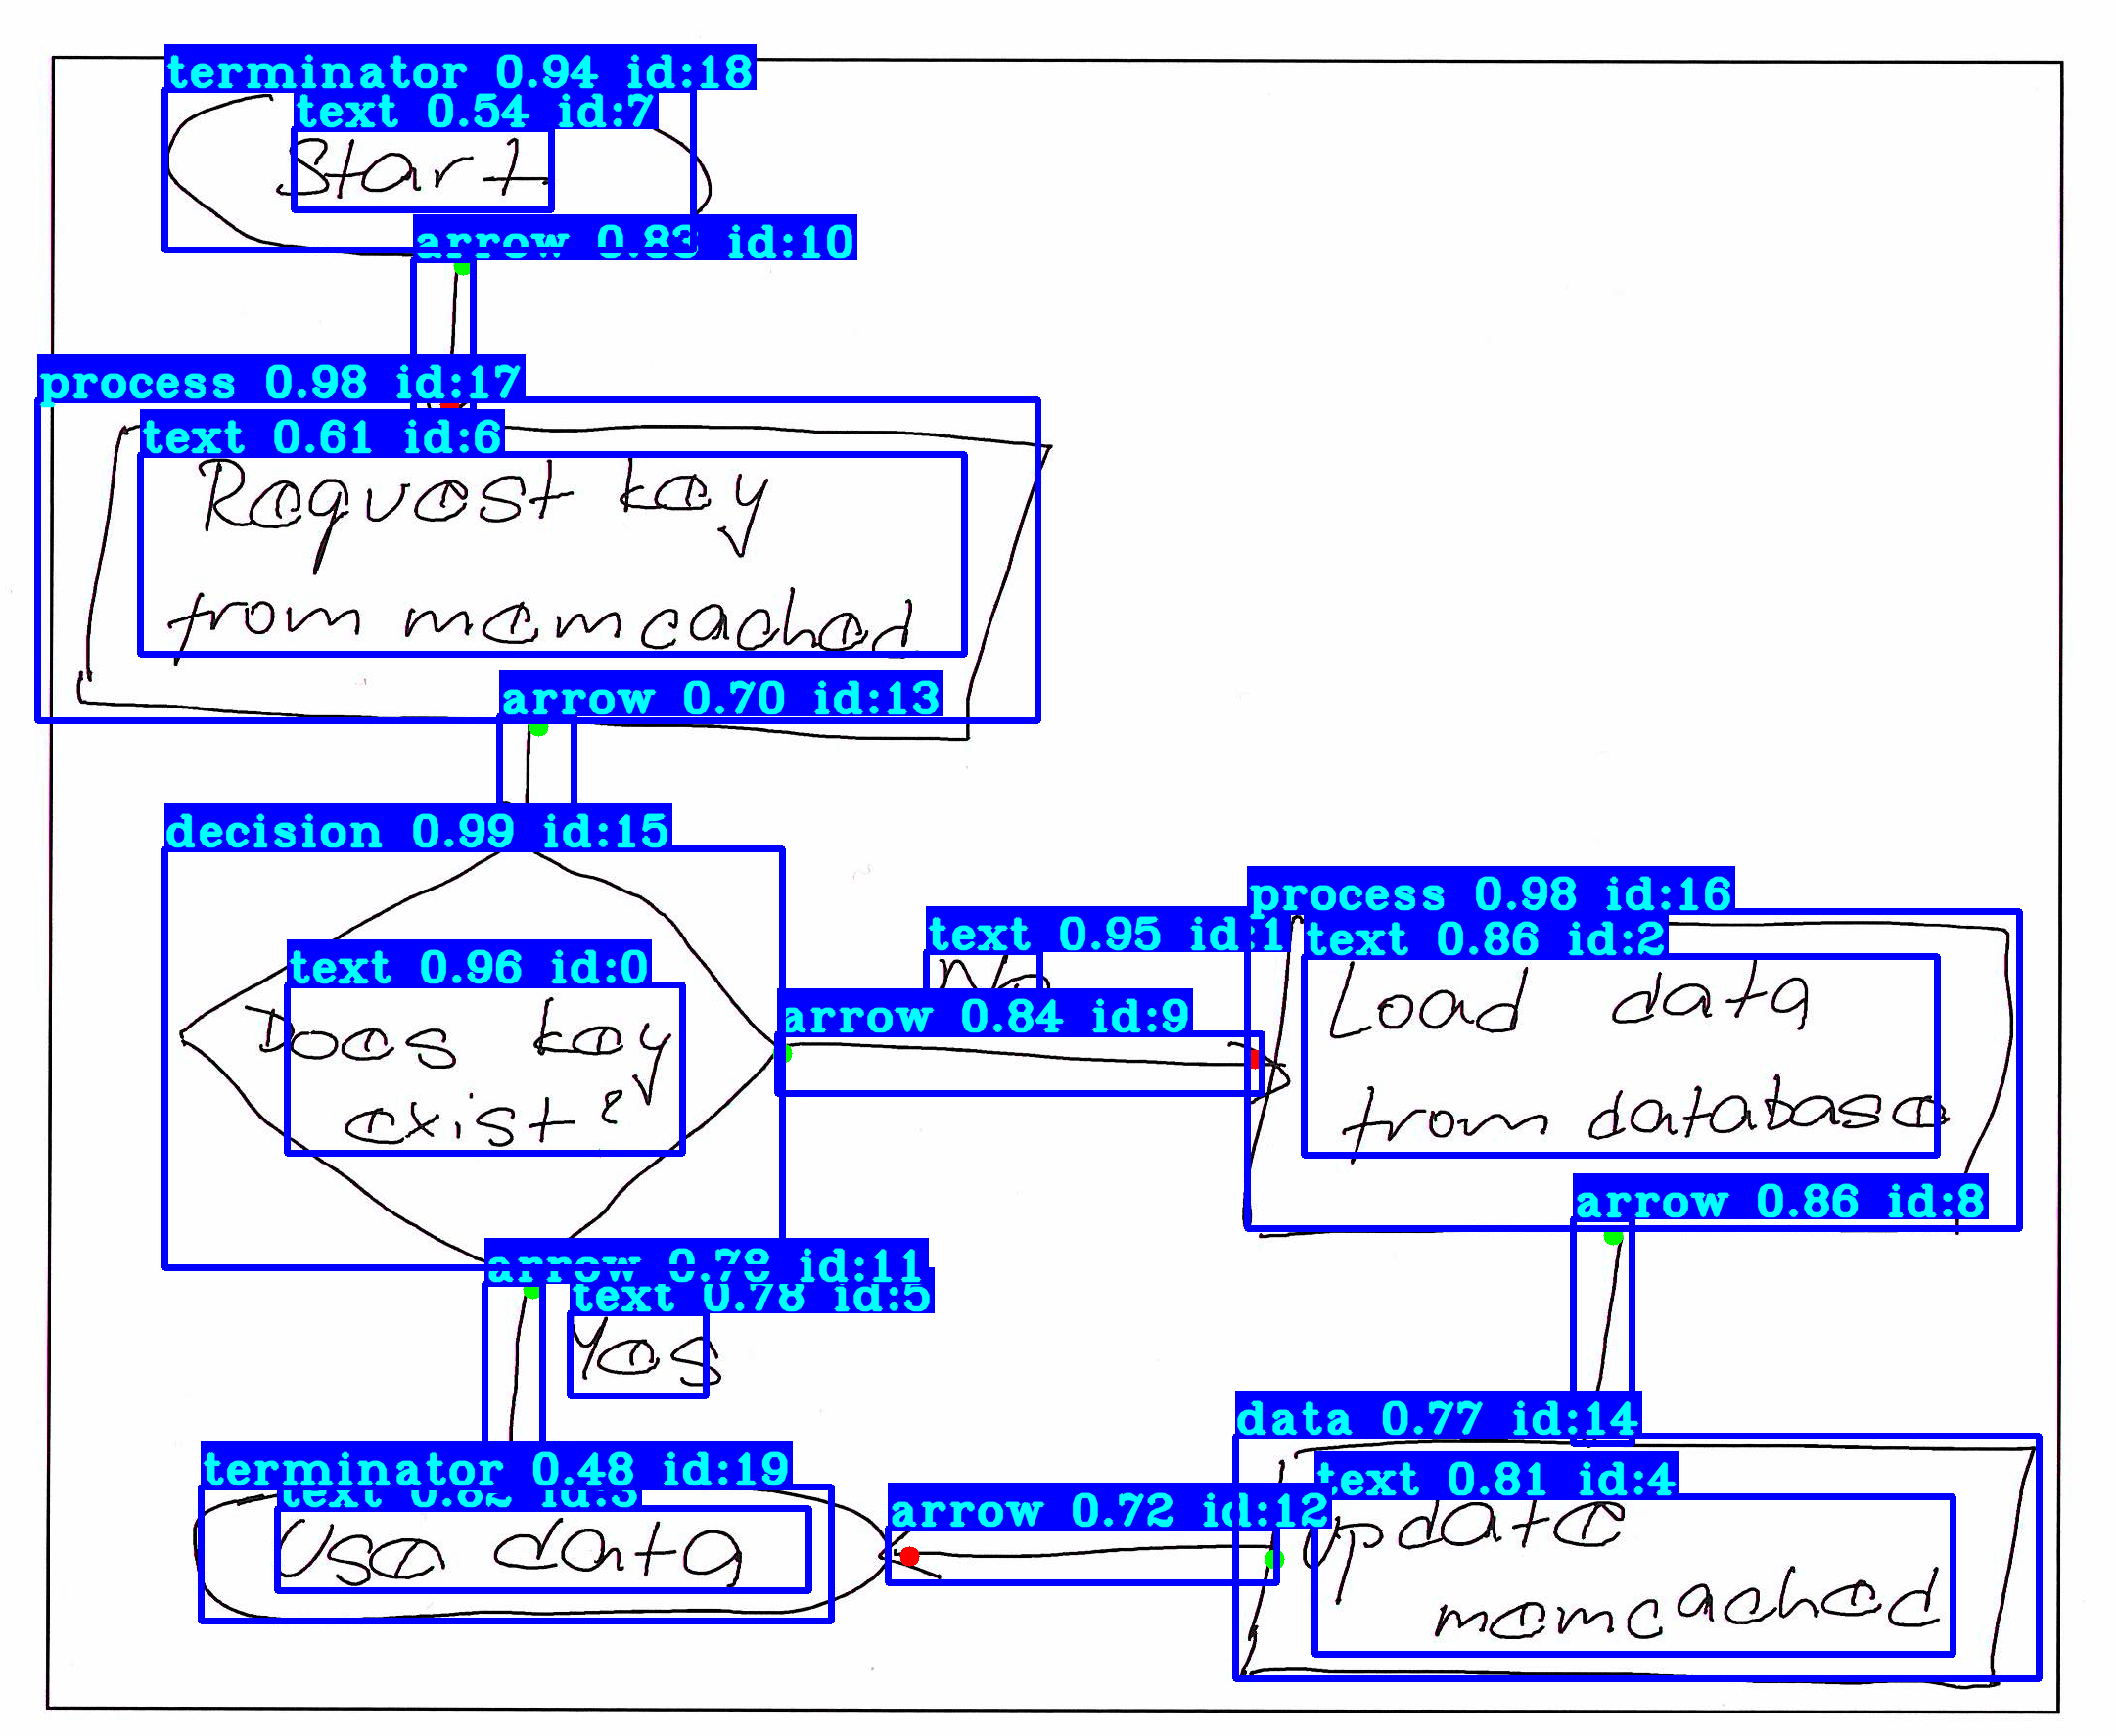
\includegraphics[width=\columnwidth]{sample.png}
\end{subfigure}
\begin{subfigure}{0.28\columnwidth}
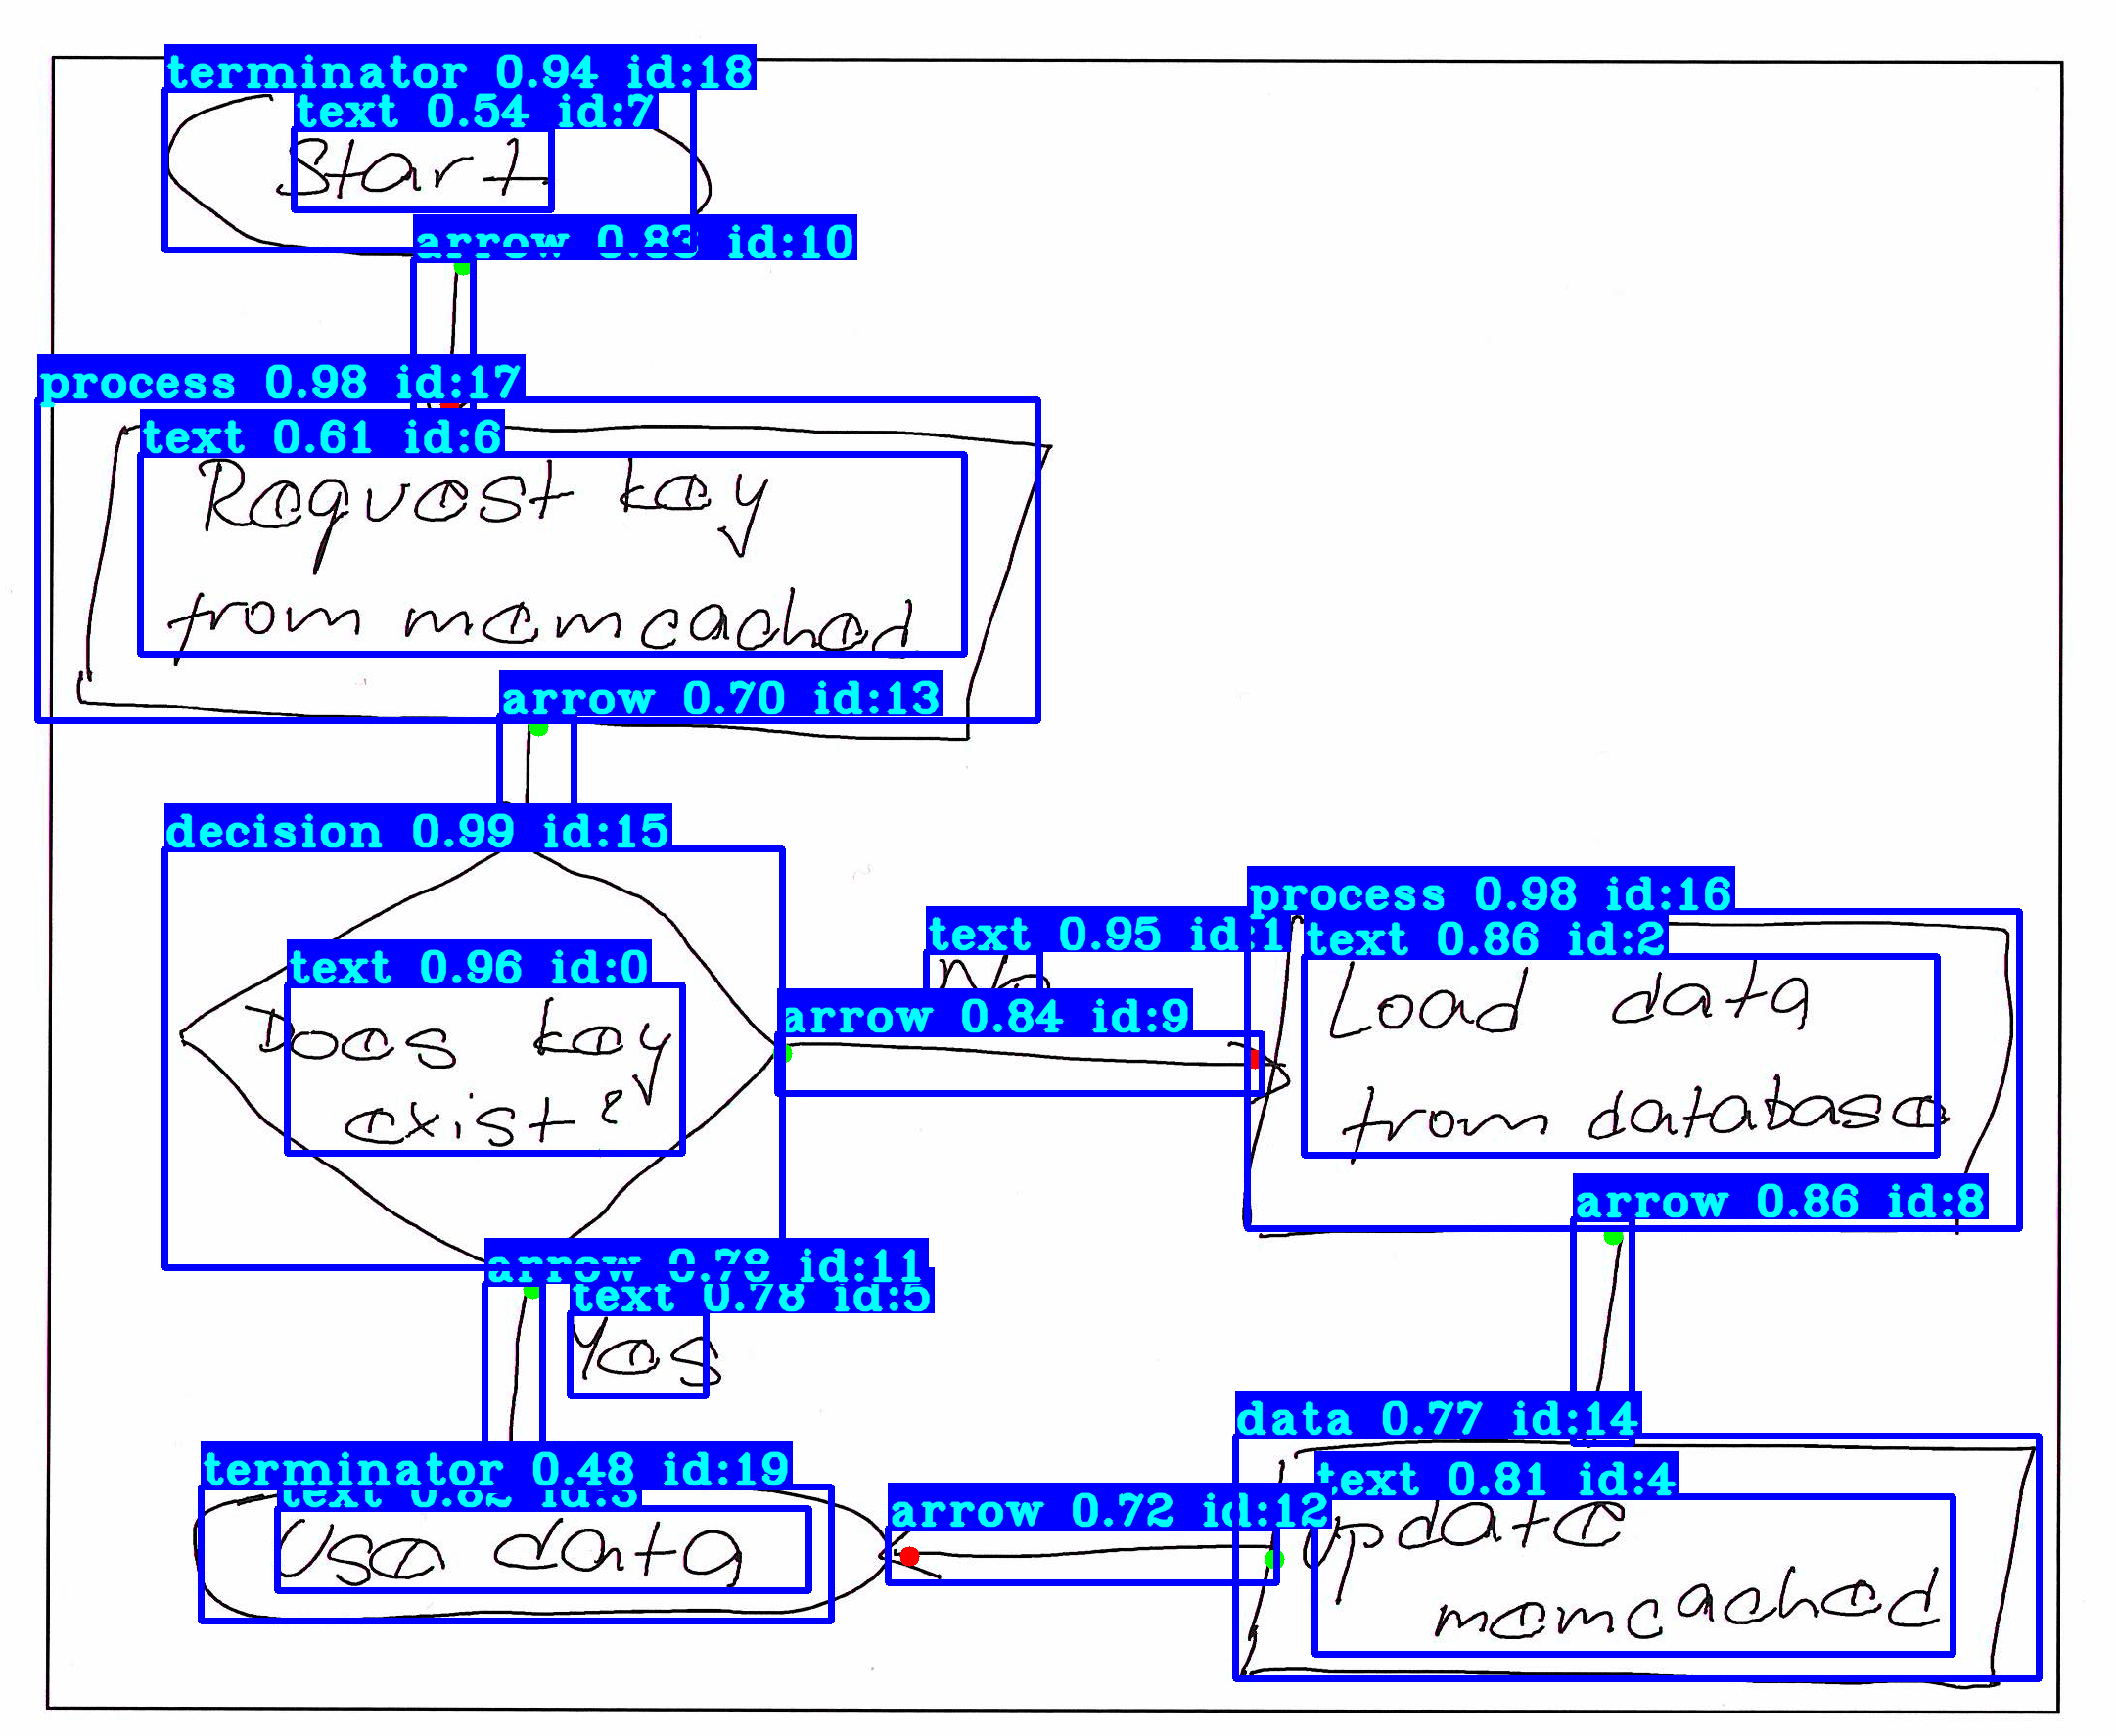
\includegraphics[width=\columnwidth]{sample.png}
\end{subfigure}
\begin{subfigure}{0.28\columnwidth}
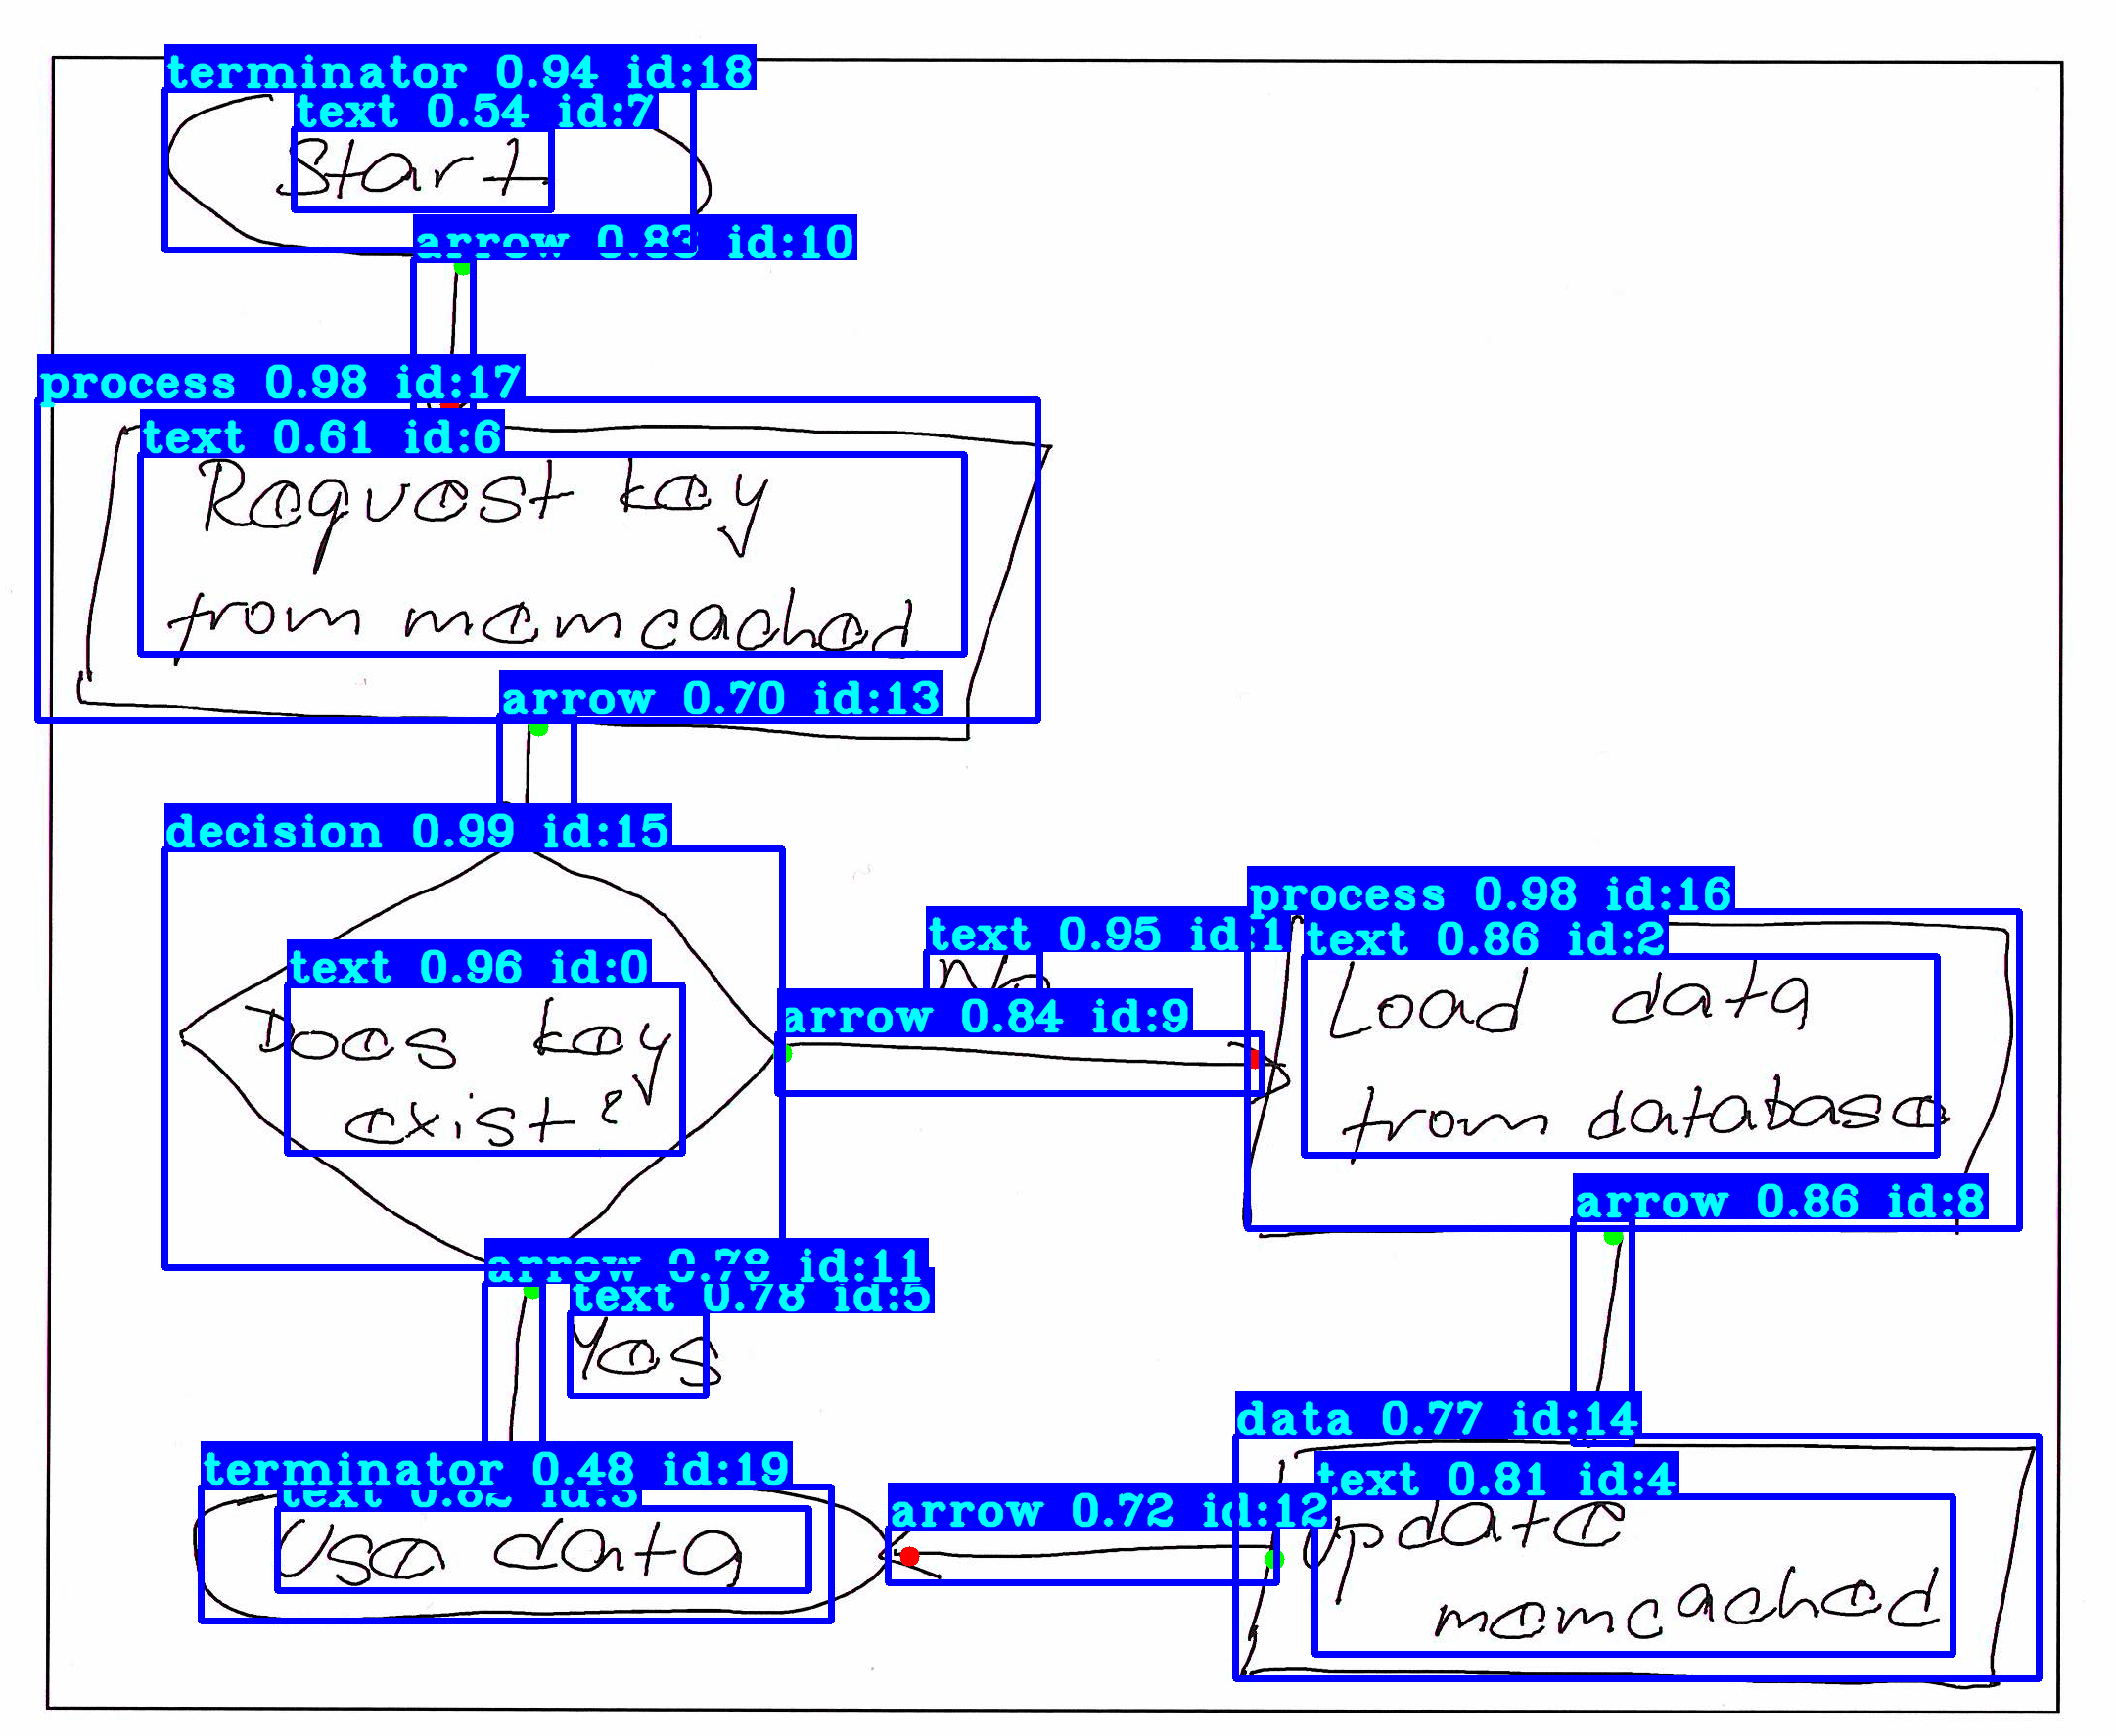
\includegraphics[width=\columnwidth]{sample.png}
\end{subfigure}
\end{figure}

In this project, we developed a program to recognize hand-drawn flowcharts.
and render them in productivity applications including word processors
and presentation softwares.

Many softwares support the creation of flowcharts through providing
drawing primatives such as circles, blocks, and arrows,
they are often awkward to use. Many people avoid flowcharts due to such
difficulty, despite flowcharts are versatile and are often the best and most
succinct waay to summarize concepts such as workflow
and relationships. We sought to offer a solution to this problem.

We developed a deep learning model that takes take an image
of a flowchart, and extract the blocks, text, arrows, and their relative
positioning.
Thereafter, the flowchart can be recreated in graphical applications.
Our approach was built on \textsc{yolo-v4}
trained on objects specific to flowchart
detection, including blocks (processes), parallelograms (data),
diamonds (decisions), circles (I/O), arrows, and lines.
We also extract text elements and converted to text using Tesseract
\textsc{ocr}. The following are technical details of our implementation.

\begin{itemize}
\item Our \textsc{yolo} was trained on a dataset with 600 annotated flowchart
images, with custom \textsc{xml} preprocessing.
\item Our model was trained to detect seven custom classes (\texttt{text}, \texttt{arrow}, \texttt{data}, \texttt{decision}, \texttt{process}, \texttt{terminator}, and \texttt{connection}), starting with
pre-trained \textsc{yolo} weights. Training took a total of six hours with
\textsc{GPU}, achieving an \textsc{mAP} of $90.365\%$.
\item During post-processing, we compile a list of detected objects with a
rich set of attributes, including position, size, object class, and confidence.
\item We implemented a custom algorithm to detect arrow direction, using
\textsc{openCV}. We also established the logical connections between directed
edges and flowchart elements.
\item Text elements were identified and converted to actual text using
Google's \textsc{tesseract-ocr} engine.
\item We then follow the logical order of arrows to render the flowchart
elements in order.
\item Finally, to demonstrate  using \textsc{SchemaDraw} as the drawing application.
\item We utilized the following tools in the project: \textsc{python 3},
\textsc{openCV 2}, \textsc{Pytorch 2.0}, scripts from PyLessons,
Google Colab (faster \textsc{GPU}-based training,
\textsc{yolo-v4}, Google \textsc{tesseract}, and
\textsc{schemaDraw}.
\end{itemize}


In conclusion,
we have successfully implemented a \textsc{yolo-v4} based program to
recognize hand-drawn flowcharts, and demonstrated the effectiveness of our
method.

% \subsection*{Contributions}

\begin{table}[htbp]
\centering
\begin{tabular}{|c|c|c|c|c|c|c|c|}
\hline
Name & Major \& ID & Main Responsibility & \textsc{C} &
	\textsc{T\&V} & \textsc{P} & \textsc{ES} & Overall \\
\hline
Mu Chen & SE, 014725425 & R\&D, \textsc{yolo}, \textsc{schemaDraw} & $40\%$ & $40\%$ & $10\%$ & $10\%$ & $25\%$ \\
Roger Kuo & SE, 013784706 & R\&D, \textsc{yolo}, arrow detection & $40\%$ & $40\%$ & $10\%$ & $10\%$ & $25\%$ \\
Hardy Leung${}^\star$ & AI, 016711877 &
Proposal, Summary, Coordinator & $10\%$ & $10\%$ & $10\%$ & $70\%$ & $25\%$ \\
Jasmine Wang & AI, 002805362 & testing, presentation & $10\%$ & $10\%$ & $70\%$ & $10\%$ & $25\%$ \\ \hline
\end{tabular}
\caption{\textsc{C} = coding, \textsc{TV} =
testing and verification,
\textsc{P} = PPT, \textsc{ES} = executive summary. $\star$ Project Coordinator.
}
\end{table}

% \bibliographystyle{acm}
% \bibliography{paper}

\end{document}
